\documentclass[10pt,a4paper]{article}
\usepackage[utf8]{inputenc}
\usepackage{amsmath}
\usepackage{amsfonts}
\usepackage{amssymb}
\usepackage{natbib}
\usepackage{graphicx}

\title{XOR single-layer model theory}
\author{Max Cotton}
\date{}

\begin{document}

\maketitle

\section{Setup}
\begin{itemize}
    \item Where the weights W11, W12, W21 and W22 are together in an array W1, as the hidden weights
    \item Weights W3 and W4 are together in array W2, as the output weights
    \item Z11 and Z12 are together in an array Z1, and is the dot product of the W1 array and the input array, summed with a bias 
    \item A1 is sigmoid(Z1)
    \item Z2 is the dot product of the W2 array and A1, summed with a bias
    \item A2 is sigmoid(Z2), which is the prediction Y
\end{itemize}

\section{Forward Propagation}

\section{Back Propagation}

% \maketitle
% \begin{figure}[h!]
% \centering
% 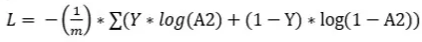
\includegraphics[width=0.3\textwidth]{src/images/cost-function.png}
% \caption{Cost Function}
% \end{figure}

\end{document}